\newpage
\subsection{Supper approximation of $x^2$ via composition}
We consider a set of equidistant girds $\Omega_\ell$ of level $\ell$ on the unit interval $\bar{\Omega}=[0,1]$ and mesh length $h_\ell = 2^{-\ell}$. The grid points $x_{\ell,i}$ are given by
\begin{equation}
x_{\ell,i}:=ih_\ell,\quad 0\le i\le 2^\ell.
\end{equation} 

A key observation about the connections between linear finite element functions and ReLU DNNs in \cite{he2020relu} is that
\begin{equation}\label{def_g}
g(x) = 2{\rm ReLU}(x) - 4{\rm ReLU}({x-\frac{1}{2}}) + 2{\rm ReLU}(x-1)\in {{\rm DNN}}_{1}^{3},
\end{equation}
for $x \in \mathbb{R}$. The nodal basis functions on $\Omega_\ell$ are defined as
\begin{equation}
\phi_{\ell,i}(x):=
\begin{cases}
g\left(\frac{x-(i-1)h_\ell}{2h_\ell}\right)\quad &x\in [x_{\ell,i}-h_\ell,x_{\ell,i}+h_\ell],\\
0 \quad &\text{otherwise}.
\end{cases}
\end{equation}
By definition, we have $\phi_{1,1}(x) = g(x)$ for $x \in[0,1]$. Besides, for $\ell=0$, we have these next two basis functions
\begin{equation}\label{key}
\phi_{0,0} = 1- x \quad \text{and} \quad \phi_{0,1} = x, \quad \forall x \in [0,1].
\end{equation}

These basis functions are used to define the piecewise linear function space
\begin{equation}
V_\ell :=\mbox{span}\{\phi_{\ell,i}: 0 \le i\le 2^\ell\} .
%\subset H_0^1(0,1).
\end{equation}
Then, let's define the the piecewise linear interpolation on $\Omega_\ell$ as:
\begin{equation}
\Pi_\ell u = \sum_{i=0}^{2^\ell}u(x_{\ell,i}) \phi_{\ell,i}. 
\end{equation}
Thus, we also have the next so-called hierarchical decomposition for $L \ge 1$
\begin{equation}
\begin{aligned}
\Pi_L u(x) &=\Pi_0 u +  \sum_{\ell=1}^L  (\Pi_\ell - \Pi_{\ell-1})u \\
&=\Pi_0 u +  \sum_{\ell}^L \sum_{i\in I_\ell}\mu_{\ell,i}\phi_{\ell,i},
\end{aligned}
\end{equation}
where
\begin{equation}
I_\ell = \{i\in \mathbb{N}~:~1\le i\le 2^\ell-1, ~i ~\text{ is odd} \}.
\end{equation}
Furthermore, we have 
\begin{equation}\label{key}
(\Pi_\ell - \Pi_{\ell-1})u = \sum_{i\in I_\ell}\mu_{\ell,i}\phi_{\ell,i} = \sum_{i\in I_\ell} \left( u(x_{\ell,i}) - \frac{1}{2}\left( u(x_{\ell,i-1})  + u(x_{\ell,i+1})  \right) \right)\phi_{\ell,i}.
\end{equation}

The key observation here is that there exist a special decomposition form once we take $u(x) = x^2$. 
By the hierarchical decomposition above, we have
\begin{equation}
\begin{aligned}
(\Pi_{\ell} - \Pi_{\ell-1})u &= \sum_{i\in I_\ell}\left( u(x_{\ell,i}) - \frac{1}{2}\left( u(x_{\ell,i-1})  + u(x_{\ell,i+1})  \right) \right)\phi_{\ell,i}(x)\\
&=\sum_{i\in I_\ell}\left(x_{\ell,i}^2 - \frac{1}{2}(x_{\ell,i-1}^2 + x_{\ell,i+1}^2)\right)\phi_{\ell,i}(x)\\
&= \sum_{i\in I_\ell}\left(x_{\ell,i}^2 - \frac{1}{2}\left((x_{\ell,i}-h_\ell)^2 + (x_{\ell,i}+h_\ell)^2\right) \right)\phi_{\ell,i}(x) \\
&=-h_\ell^2\sum_{i\in I_\ell}\phi_{\ell,i}(x).
\end{aligned}
\end{equation}
Note $\Pi_0 u = u(0)\phi_{0,0} + u(1)\phi_{0,1} = x$, we have
\begin{equation}
\Pi_L u = \Pi_0 u + \sum_{\ell=1}^L  (\Pi_\ell - \Pi_{\ell-1})u = x -\sum_{\ell=1}^\ell h^2_\ell \sum_{i\in I_\ell}\phi_{\ell,i}(x) = x -\sum_{\ell=1}^\ell h^2_\ell g_\ell(x),
\end{equation}
where
\begin{equation}\label{key}
g_\ell(x) := \sum_{i\in I_\ell}\phi_{\ell,i}(x).
\end{equation}

By definition, we have the next diagram of $g_\ell(x)$:
\begin{figure}[h!]
	\centering
	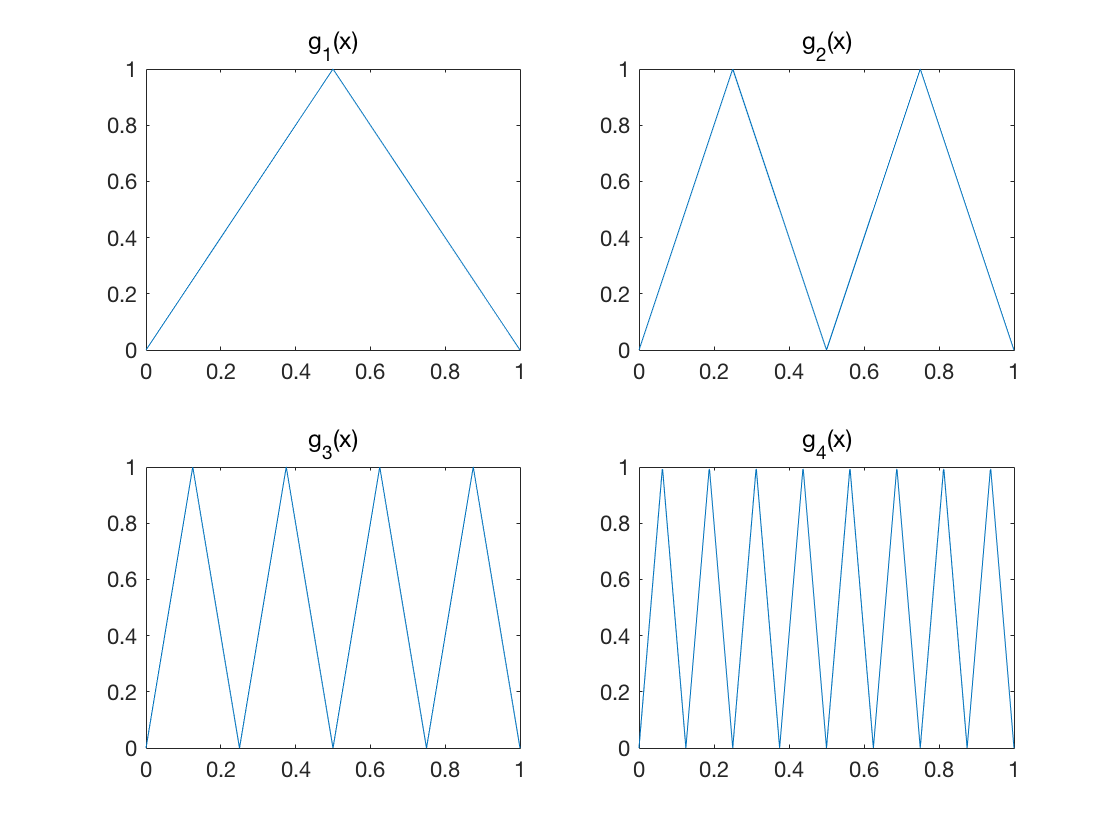
\includegraphics[width=0.6\textwidth]{figures/hierachybasis_gl}
	\caption{The figure of $g_\ell(x)$}
	\label{fig:gl}
\end{figure}

The next property plays the crucial role for the connection between ReLU DNN and hierarchical basis functions:
\begin{equation}\label{func:glinduction}
g_\ell(x)=g(g_{\ell-1}(x)),\quad \ell=2,...,L, \quad \forall x \in [0,1],
\end{equation}
with $g_1(x) = g(x)$ as defined in~\ref{def_g}. Thus, we have the next key relation by the  property of composition
\begin{equation}\label{key}
g_\ell \in {\rm DNN}_\ell^{3}.
\end{equation}
Based on the definition of $\widehat{{\rm DNN}}_{\ell}^{3}$, the above relation leads to 
\begin{equation}\label{key}
x -\sum_{\ell=1}^L h^2_\ell g_\ell(x) \in \widehat{{\rm DNN}}_{L}^{3},
\end{equation}
where $f \in \widehat{{\rm DNN}}_{L}$ is a modified DNN structure as:
\begin{equation}\label{def:ReLUDNN2}
\begin{cases}
f^{1}(x) &= \sigma \circ \theta^1 (x) \\
f^{\ell}(x) &= \sigma \circ  \theta^{\ell} ([x, f^{\ell-1}(x)]) \quad \ell = 2:L \\
f(x) &= \theta^{L+1}( [x, f^1, \cdots, f^L] ) \\
\end{cases}.
\end{equation}


